\setchapterpreamble[u]{\margintoc}
\chapter{Enriching the classic TTO formulation with advanced mechanical constraints}
Introduction
\section{Local buckling and kinematic compatibility constraints}

\subsection{Local and topological buckling constraints}

\subsection{Kinematic compatibility constraints}

\subsection{Minimum slenderness constraints}
As precedently seen, one of the limit of the tto is that is based on truss model. so we cannot trust the results if the model is outside of his limits. For that reason in section we have already set the limit to 15. th focus of this section is to introduce an upper bound on the cross sectional area design variable to deal with that

we first formely introduce the slenderness of a bar as:
\begin{equation}
    \lambda = \frac{\ell}{R_{\mathrm{g}}}
\end{equation}

remembering that
$R_{\mathrm{g}} = \sqrt{I/a_j}$ $I = \pi r_j^4/4$ 
$a_j=$
\begin{equation}
    R_{\mathrm{g}} = r/2
\end{equation}

The minimum slenderness limit constraints $\vect{g}_{\text{slend}}$ are stated as:
\begin{equation}
    a_j \leq \frac{4 \pi \ell_j^2}{\lambda_{\text{max}}}, \quad \forall j \in [1,\ldots, N_{\text{el}}]
\end{equation}

we re run the optimization on the l shape beam of section XX using formulation and adding only the slenderness constraints. in image the results of st = 1,08,03,02. we see how the same load is repartitioned on multiple bars. we active more bars because there is un upper imit on the area (and then the force ) that they can bear.

\begin{figure*}[]
    \subcaptionbox{}{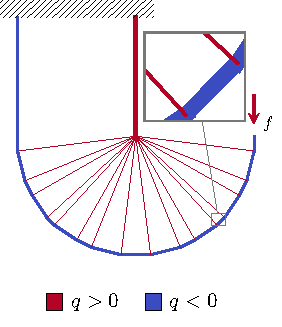
\includegraphics[width=0.23\linewidth ]{figures/04_TTO_improvements/00_slend_sol/1_opt.pdf}}
    \hfill
    \subcaptionbox{}{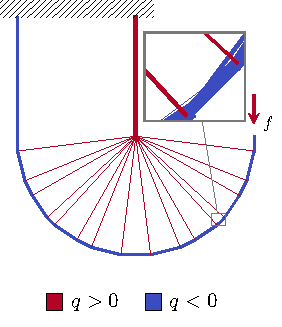
\includegraphics[width=0.23\linewidth ]{figures/04_TTO_improvements/00_slend_sol/08_opt.pdf}}
    \hfill
    \subcaptionbox{}{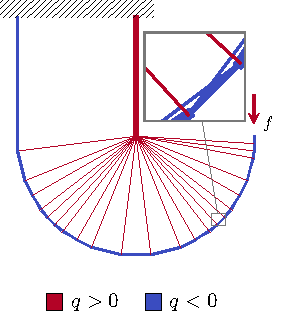
\includegraphics[width=0.23\linewidth ]{figures/04_TTO_improvements/00_slend_sol/03_opt.pdf}}
    \hfill
    \subcaptionbox{}{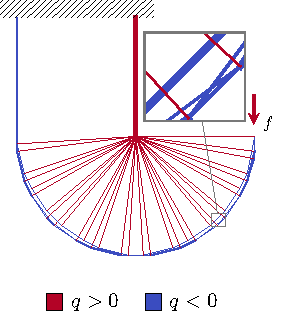
\includegraphics[width=0.23\linewidth ]{figures/04_TTO_improvements/00_slend_sol/02_opt.pdf}}
    \caption{\todo{todo} 34 38 56 79}
    \label{fig:04_tto_slend}
\end{figure*}

We compared the results with the olds . we see that the number of active bars increase, as the colaulation time, but the volume stays almost the same, indicating that there are plenty of solutions with almost the same volume

\begin{table*}[]
    \centering
    \sisetup{table-auto-round}
    \begin{tabular}{S[table-format = 2.1]
                    S[table-format = 2.2]
                    S[table-format = 2.1] 
                    S[table-format = 2.2]
                    S[table-format = 2.1]                    
                    S[table-format = 1.4]
                    S[table-format = 1.2]
                    S[table-format = 1.2]}
                    \toprule
    $\bm \sigma_L$&$\bm V_\text{f}$  & {\textbf{Min} $\bm \lambda$} & $\bm V_\text{f,sl}$  & {\textbf{Min} $\bm \lambda_\text{sl}$}&$\bm V_\text{f,sl}/\bm V_\text{f}$&$\bm N_\text{el,sl}/\bm N_\text{el}$&$\bm t_\text{sl}/\bm t$\\ \midrule
    1           & 6.208431\ppercent  & 15.795                    & 6.208431\ppercent& 15.795  &1&1       &1.02            \\
    0.90        & 6.898257\ppercent  & 14.984                    & 6.898257\ppercent& 14.984  &1&1       &1.03            \\
    0.80        & 7.760539\ppercent  & \color{accent_r_1}14.127  & 7.761069\ppercent& 15.0    &1,0000682&1,1176       & 2.27    \\
    0.70        & 8.869187\ppercent  & \color{accent_r_1}13.215  & 8.870386\ppercent& 15.0    &1,0001351&1,1176       & 2.21    \\
    0.60        & 10.347385\ppercent & \color{accent_r_1}12.235  &10.349476\ppercent& 15.0    &1,0002020&1,1176      & 1.12    \\
    0.50        & 12.416862\ppercent & \color{accent_r_1}11.169  &12.420203\ppercent& 15.0    &1,0002690&1,1176      & 1.07    \\
    0.4         & {--}      & {--}                               &15.526292\ppercent& 15.0    &{--}&{--} &{--}                 \\
    0.3         & {--}      & {--}                               &20.705531\ppercent& 15.0    &{--}&{--} &{--}        \\ 
    0.2         & {--}      & {--}                               &31.061628\ppercent& 15.0    &{--}&{--} &{--}                \\ \bottomrule
    \end{tabular}
    \caption{\todo{todo}}
    \label{tab:my-table}
\end{table*}








\section{Optimization formulation and solving strategy}

\subsection{Optimization strategy}

\subsection{First step: SLP optimization}

\subsection{Handling local minima: reinitialization strategy}

\subsection{Second step: NLP optimization}

\section{Numerical application}

\subsection{Ten-bar truss}

\subsection{2D cantilever beam}

\subsection{Simply supported 3D beam}

\subsection{Ten-bar truss with multiple load cases}

\section{Conclusion}